This section will show you how to add data to the \gdcase{} we just created, using an Excel file. 
\begin{enumerate}
\item In the \gdtestcaseeditor{}, select the \bxname{TestAdder} \gdcase{}. In the \gdpropview{}, you can see the parameters this \gdcase{} has. 
\item Open Excel and set up a worksheet whose worksheet name is the language code for your \gdaut{} language (in this case, en\_US). Enter the parameter names into the top sheets of the worksheet, and enter values for them as shown in the example table (\bxfigref{TutExcelTable}).

\begin{figure}[h]
\begin{center}
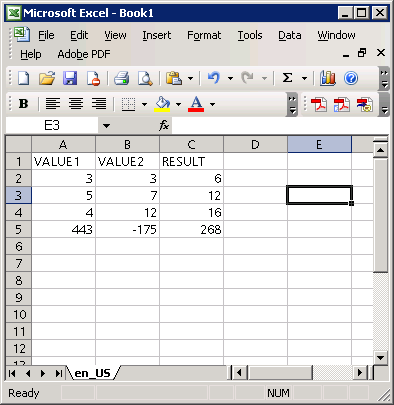
\includegraphics{Tutorials/PS/TutExcelTable}
\caption{Example Excel Table}
\label{TutExcelTable}
\end{center}
\end{figure}

\item Save the worksheet into your workspace directory. 
\item  Enter the name of the Excel file in the \bxname{Excel Data File} field in the \gdpropview{} and save the \gdcase{}. 

\bxtipp{If you look in the \app{} preferences:\\
\bxmenu{Window}{Preferences}{GUIdancer}\\
you will see that the workspace directory is the default directory for test data. You could define a different one if you wanted to.} 
\end{enumerate}
